\subsubsection{Employer Branding}\label{employer_branding}
%Philipp

%\gls{eB}    % employerBranding
%\gls{cI}    % companyImage
%\gls{tJS}   % totalJobSatiscation

The employerBranding (eB) is the score which is reported to the external world in order to measure the value of the company as an employer in total. This score is comparable to the total score for companies which is presented on websites like kununu or glassdoor. The employer branding is a combined score out of the Job Satisfaction and the Company Image. As the Company Image implicitly incluences the Job Satisfaction rating it is weighted with 0.4 in the calculation of the employer branding score. The general formula is
\begin{center}
\texttt{eB = 0.4 * cIS + 0.6 * tJS} \\
\texttt{with} \\
\texttt{cI = companyImage}   \\
\texttt{tJS = totalJobSatisfactione}
\end{center}

In order to make the employer branding rating more realistic, we need to think about extreme cases where either the employee satisfaction or the company image is rated very low. The usage of a simple weighted average would have the effect that values of $tJS = 100$ and $cI = 0$ lead to an overall score of 60.
Therefore we need to include an indicator function which incorporates a punishment for smaller values.
This can be done by incorporating a multiplier which is based on an IF statement. See the \textit{Excel} implementation below:
\begin{center}
    $=ROUND(((0.4*cI+0.6*tJS)*IF(cI<30,0.5,IF(cI<60,0.8,IF(cI>60,1))))/10,0)$
\end{center}

The following pseudo code explains the statement above.

\begin{itemize}
    \item score = 0.4*CI + 0.6*tJS
    \item IF CI $\leq$ 30 THEN Employer Branding = Employer Branding * 0.5
    \item ELSEIF CI $\leq$ 60 THEN Employer Branding = Employer Branding * 0.8
    \item ELSEIF CI $\geq$ 60 THEN Employer Branding = Employer Branding * 1
\end{itemize}

By this we ensure a sufficient punishment of the overall Employer Branding score. To achieve this we need to create a matrix and a 3D graph to visualize the possible implications on the employer branding. Graphic \ref{img:EBS} shows the implications of the two input parameters on the Employer Branding.

\begin{figure}
	\centering
	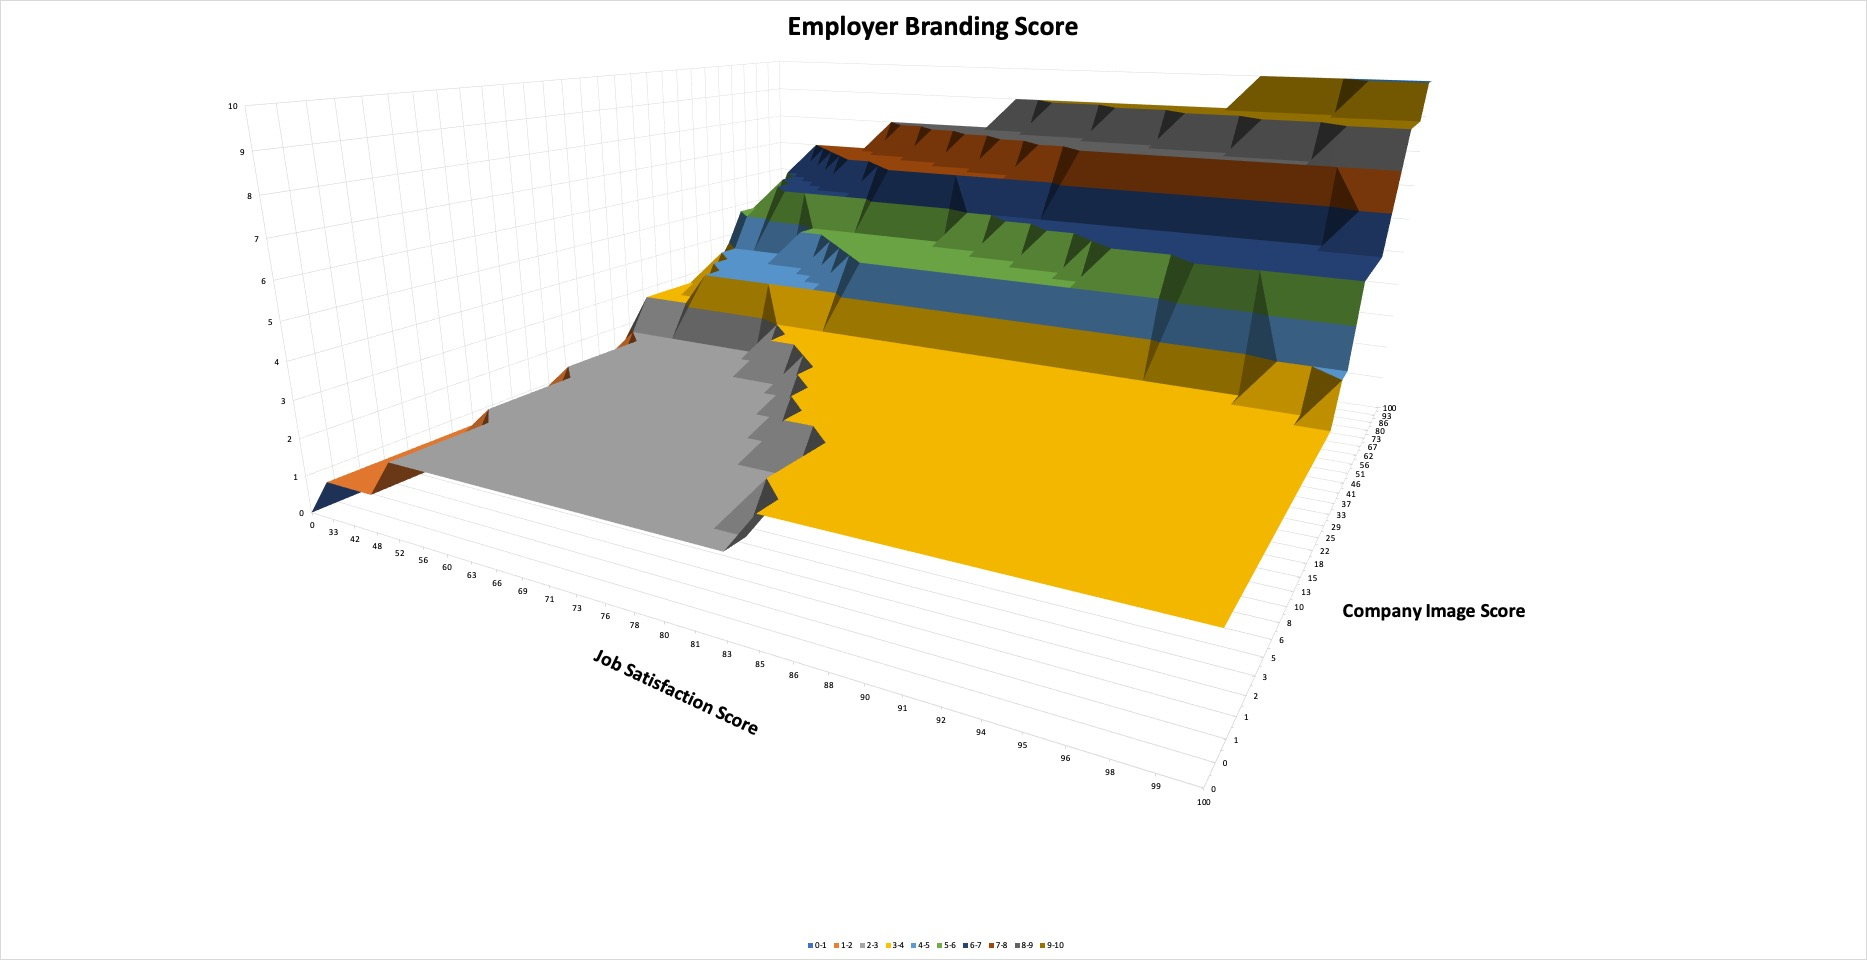
\includegraphics[width=12.5cm]{images/EBS.jpg}
	\caption{Employer Branding Score Calculation}
	\label{img:EBS}
\end{figure}